\section{評価実験}\label{sec:experiment}
本章では，方策再利用の枠組みの下で方策選択手法
（Boltzmann，$\varepsilon$-greedy，UCB）を比較し，
さらに報酬設計を2種類用意して報酬構造の違いによる影響も検証する．

\subsection{実験設定}
格子状迷路を用い，行動は上下左右とする．
壁衝突時は状態が遷移しない．
各エピソードはスタートから開始し，ゴール到達で終了する．
転移設定として，ソース側で学習した方策を方策ライブラリ 
$\mathcal{L}$ に格納し，
ターゲットでは各エピソード開始時に
 $\mathcal{L}\cup\{\pi_{\mathrm{new}}\}$ 
 から1つを選択して実行する．
なお，環境をドメイン $D=\langle S,A,T\rangle$ と
タスク $\Omega=\langle D,R_{\Omega}\rangle$ に分け，
本研究では同一ドメイン $D$ を共有する複数タスク
（ゴール設定・報酬設計の違い）を対象とする．
方策選択は Boltzmann，$\varepsilon$-greedy，
UCB の3手法を比較し，各方策 $\pi_i$ 
について推定価値 $V_i$ と選択回数 $N_i$ を保持して，
エピソード終了後にリターンに基づいて $V_i$ を更新する．
また，エピソード内は再利用率 $\psi$ による 
$\pi$-reuse を用いて行動を決定する．
報酬設計は2条件とし，
(i) ゴール到達報酬のみ（報酬設計1），
(ii) 報酬設計1に加えてステップ負報酬と壁衝突ペナルティを導入（報酬設計2）とした．

\begin{figure}[!b]
  \centering
  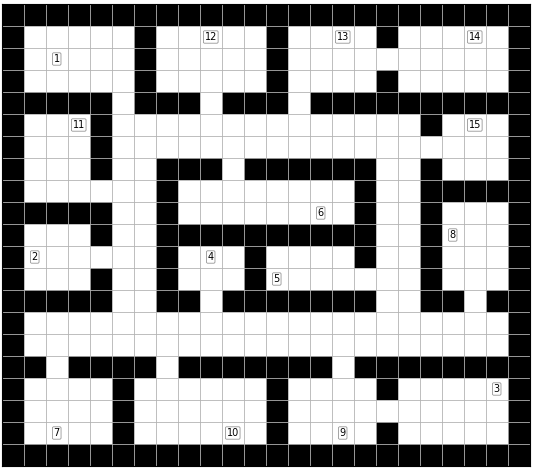
\includegraphics[width=0.80\columnwidth]{../contents/figure/maze.png}
  \caption{迷路環境と各タスクのゴール位置}
  \label{fig:maze}
\end{figure}


\subsection{評価方法}
各trial（episode）$k$で得られる割引累積報酬を 
$W_k$ とし，trial $t$ までの累積平均利得
\begin{equation}
\bar{W}_t=\frac{1}{t}\sum_{k=1}^{t} W_k
\end{equation}
を学習曲線として用いる．実験はソース側で学習した方策を
 $\mathcal{L}$ に格納した後，
ターゲットで各エピソード開始時に方策選択手法により 
$\mathcal{L}\cup\{\pi_{\mathrm{new}}\}$ 
から方策を選択して実行し，
エピソード終了後に推定価値の更新とQ学習による
 $\pi_{\mathrm{new}}$ の更新を繰り返す．
上記を報酬設計1/2の2条件で実施し，3手法の結果を比較する．
